\id{МРНТИ 28.23.17}

{\bfseries КЛАССИФИКАЦИЯЛЫҚ АЛГОРИТМДЕРДІ ҚОЛДАНЫП ДАУЫСТЫ ТАНУ}

{\bfseries \textsuperscript{1}Н.О.Мекебаев}
\begin{figure}[H]
	\centering
	
\includegraphics[width=0.8\textwidth]{media/ict/image1}
	\caption*{}
\end{figure}

\begin{figure}[H]
	\centering
	
\includegraphics[width=0.8\textwidth]{media/ict/image1}
	\caption*{}
\end{figure}

{\bfseries , \textsuperscript{1}Н.А. Модовов}
\begin{figure}[H]
	\centering
	
\includegraphics[width=0.8\textwidth]{media/ict/image1}
	\caption*{}
\end{figure}

\textsuperscript{1}Ж.А.
\begin{figure}[H]
	\centering
	
\includegraphics[width=0.8\textwidth]{media/ict/image1}
	\caption*{}
\end{figure}


\textsuperscript{1}Қазақ ұлттық қыздар педагогикалық университеті,
Алматы, Қазақстан

\textsuperscript{2}Әл-Фараби атындағы Қазақ ұлттық университеті, Алматы,
Қазақстан

{\bfseries \textsuperscript{\envelope }}Корреспондент-автор:
\href{mailto:nurbapa@gmail.com}{\nolinkurl{nurbapa@gmail.com}}

Дауыс тану жүйелері машиналық оқыту әдістеріне негізделген, оның ішінде
классификациялық алгоритмдер кеңінен қолданылады. Классификация дауыс
сигналдарын әртүрлі санаттарға, мысалы, сөздер немесе сөйлемдерге бөліп
тануды жүзеге асырады. Бұл үдерісте жиі қолданылатын алгоритмдерге
логистикалық регрессия, шешім ағаштары және нейрондық желілер жатады.
Дауыс сигналын өңдеуде алдымен ерекшеліктері, яғни маңызды параметрлері,
экстракцияланады, содан кейін олар классификаторға беріледі.
Классификация нәтижесінде жүйе сөйлеген сөзді мәтінге түрлендіреді
немесе дыбыстың нақты мазмұнын анықтайды. Бұл технология адам-компьютер
өзара әрекеттестігін жақсарту үшін маңызды. Бұл мақалада машиналық оқыту
әдістерін қолдана отырып, сөйлеушінің даусын анықтау мәселесін шешу үшін
жіктеу алгоритмдерін қарастырамыз. Сөйлеудің алдын ала өңдеуде МҒСС-ті
алгортимін пайдаландық. Жоғарыдағы мәселені шешу үшін бес жіктеу
алгортмі қарастырылып, салыстырмалы талдау жасалды. Алғашқы эксперимент
жасағанда ең жақсы нәтиже көрсеткен SVC алгортимі 0,90 және MLP
Classifier алгоритмі 0,83 нәтижелерін көрсетті. Келесі экспермиентте
жеке тұлғаның дауысын анықтауда неғұрлым үлкен дәлдікте Robust scaler
әдісімен масштабтауда -- 0,93 көпқабатты персептрон көрсете бастады.
Сондықтан бұл мәселені шешу үшін сөйлеу сигналының ерекшелігін ескеретін
көп қабатты перцептронды қолдануға болады.

{\bfseries Түйін сөздер:} алгортим, дауыс, сөйлеуді тану, ASR, MFCC, MLP.

{\bfseries РАСПОЗНАВАНИЕ ГОЛОСА С ПОМОЩЬЮ АЛГОРИТМОВ КЛАССИФИКАЦИИ}

{\bfseries \textsuperscript{\envelope  1}Н.О.Мекебаев,
\textsuperscript{2}Д.К.Даркенбаев, \textsuperscript{1}Модовов Н.А,
\textsuperscript{1}Орынтаева Ж.А.}

\textsuperscript{1}Казахский национальный женский педагогический
университет, Алматы, Казахстан

\textsuperscript{2}Казахский национальный университет им. Аль-Фараби,
Алматы, Казахстан

e-mail: \href{mailto:nurbapa@gmail.com}{\nolinkurl{nurbapa@gmail.com}}

Системы распознавания речи основаны на методах машинного обучения, среди
которых широко применяются классификационные алгоритмы. Классификация
выполняет задачу разделения голосовых сигналов на различные категории,
такие как слова или предложения. К часто используемым алгоритмам
относятся логистическая регрессия, деревья решений и нейронные сети. В
процессе обработки голосового сигнала сначала извлекаются его
особенности, то есть важные параметры, которые затем передаются
классификатору. По результатам классификации система преобразует речь в
текст или определяет конкретное содержание звука. Эта технология важна
для улучшения взаимодействия человека с компьютером. В данной статье
обсуждается алгоритм классификации для задачи идентификации речи с
использованием метода машинного обучения. Алгоритм MFCC используется для
предварительной обработки речи. Для решения этой задачи проведен
сравнительный анализ пяти алгоритмов классификации. В первом
эксперименте были определены методы опорного вектора -- 0,90 и
многослойного перцептрона -- 0,83 и показаны лучшие результаты. Во
втором эксперименте был предложен многослойный перцептрон с точностью
0,93 с использованием метода Робастного скалера для идентификации
личности. Поэтому для решения этой проблемы можно использовать
многослойный персептрон, учитывающий детали аудиосигнала.

{\bfseries Ключевые слова:} алгортим, голос, распознавание речи, ASR, MFCC,
MLP.

{\bfseries VOICE RECOGNITION USING CLASSIFICATION ALGORITHMS}

{\bfseries \textsuperscript{\envelope 1}N.Mekebayev \textsuperscript{\envelope },
\textsuperscript{2}D.Darkenbayev, \textsuperscript{1}N.Modovov,
\textsuperscript{1}Zh.Oryntaeva.}

\hl{\textsuperscript{1}}Kazakh National Women' s
Pedagogical University, Almaty, Kazakhstan

\textsuperscript{2}Al-Farabi Kazakh National University, Almaty,
Kazakhstan

e-mail: \href{mailto:nurbapa@gmail.com}{\nolinkurl{nurbapa@gmail.com}}

In Speech recognition systems are based on machine learning methods,
among which classification algorithms are widely used. Classification
performs the task of dividing voice signals into various categories,
such as words or sentences. Commonly used algorithms include logistic
regression, decision trees, and neural networks. During voice signal
processing, features, i.e., important parameters, are first extracted
and then passed to the classifier. Based on the classification results,
the system converts speech into text or determines the specific content
of the sound. This technology is essential for improving human-computer
interaction.This article discusses a classification algorithm for the
problem of speech identification using the machine learning method. The
MFCC algorithm is used for preprocessing speech. To solve this problem,
a comparative analysis of five classification algorithms was carried
out. In the first experiment, the methods of the reference vector --
0.90 and the multilayer perceptron -- 0.83 were determined and the best
results were shown. In the second experiment, a multilayer perceptron
with an accuracy of 0.93 was proposed using the Robust Scaler method for
personality identification. Therefore, a multilayer perceptron can be
used to solve this problem, taking into account the details of the audio
signal. be used, taking into account the details of the audio. signal.

{\bfseries Keywords:} algorithm, voice, speech recognition, ASR, MFCC, MLP.

{\bfseries Кіріспе.} Ауыз екі сөйлеу тілін тану -- аудиодағы сөйлеуші
сөйлейтін тілді жіктеу мәселесі. Ол әдетте сөздің тілдік санатын
бастапқыда анықтау үшін, кейіннен өңдеуді жеңілдету үшін көптілді
автоматты сөйлеуді тану (ASR) сияқты көптілді сөйлеуді өңдеу
тапсырмаларының алдыңғы бөлігі ретінде пайдаланылады. Тұрақты және
сенімді тілді сәйкестендіру жүйесі бұл жүйелерде жоғары өнімділік пен
дәлдікке жетудің кілті болып табылады {[}1{]}.

Зерттеудің мақсаты сөйлеушінің дауысын анықтауға арналған машиналық
оқытудың классификациялық әдістерін зерттеу. Осы мақсатқа жету үшін
келесі міндеттер орындалды. Классификация алгоритміне салыстырмалы
талдау жүргізіліп бірқатар жіктеу алгоритмдері және сөйлеуді алдын ала
өңдеу мәселелері қарастырылды {[}2{]}.

Дәстүрлі тілдік анықтау көбінесе акустикалық және фонетикалық
ерекшеліктерге сүйенеді. Жалпы акустикалық сипаттамаларға, басқалармен
қатар, кепстральды мель-жиілік коэффициенттері (MFCC), дельта
коэффициенттері, перцептивті сызықтық болжау коэффициенттері (PLP) және
кепстральды гамма-жиілік коэффициенттері жатады {[}3{]} .

Соңғы жылдары cөйлеуді автоматты түрде тану (ASR), визуалды сөйлеуді
тану ((VST) және аудиовизуалды сөйлеуді тану (AVSR) салаларында ауқымды
ғылыми-зерттеу жұмыстары жүргізілуде {[}4{]}.

Бұл мақалада дауысты (сөйлеу екі тілді) тануды қарастырамыз. Тілді тану
-- бұл сөйлеушіні тануға ұқсас мәселе, өйткені біз белгілі бір сөздің
мазмұны туралы емес, бүкіл мәлімдеме туралы ақпарат алуға тырысамыз.
Жіктеу алгортимдері техникасындағы дауысты (тілді) тануға қолдану біздің
әдістеріміздің жан-жақты екенін және сөйлеудің бірнеше саласында
әлеуетті қолданылатынын көрсетеді {[}5{]}.

Қазақстанда қазақ тілінің сөйлеу технологиялары зерттелуде. Қазақ тілі
агглютинативті тілдер тобына жатады. Агглютинативті тілдердің
құрылымында әр түрлі форматтағы қосымшалар (жұрнақтар, жалғаулар)
бірінен соң бірі кезектесіп қосылады, бұл сөзді өзгертудің басым түрі
болып табылады және осы қосымшалардың әрқайсысы тек бір мағынамен
жүктеледі {[}6{]}. Түрік, моңғол, корей тілдері агглютинативті тілдерге
жатады. Біздің елімізде қазақ тіліндегі тұлғаны тану жүйесі әлі
дамымаған, бұл аталған бағыттағы зерттеулерді өзекті етеді.

Бұл мақалада жіктеу алгоритмдерін қолдана отырып, дауысты тану, анықтау
міндеттерін қарастырамыз.

{\bfseries \hl{Материалдар мен әдістер.}} Сөйлеуді тану үдерісі негізінде
алдын ала өңдеуден тұрады {[}7{]}. Осы мақалада біз дауыстың динамикалық
өңдеуде МҒСС-ті қолданамыз. Сөйлеу сигналының алдын-ала өңдеу үдерісі
1-ші суретте көрсетілген. MFCC (Mel-Frequency Cepstral Coefficients) мел
жиілігінің кепстральды коэффициенттері дауыс, дыбыспен жұмыс жасау
кезінде ең танымал таңдау болып табылады. Бұл тәсілдің ерекшелігі -
бастапқы сигналдың ұзындығынан алынған сипаттамалар векторы және ондағы
сөйлейтін жеке ерекшеліктердің таралуын есепке алу {[}8{]}.

\begin{figure}[H]
	\centering
	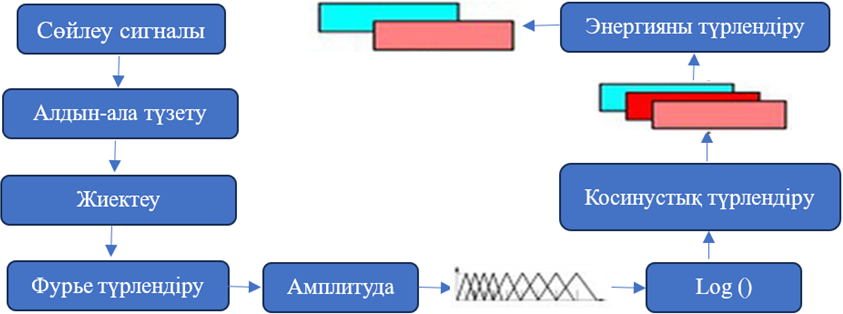
\includegraphics[width=0.8\textwidth]{media/ict/image5}
	\caption*{}
\end{figure}


{\bfseries 1-- сурет. Сөйлеу сигналын алдын ала өңдеу}

Әрбір жазылған аудио негізінде 5806 белгі алынды. Аудио файлдағы әрбір
кез-келген дауыс жазылып жатқан сигнал динамиктің белгі атымен
белгіленеді. Осы алынған дерек, мәліметтер жиынының жалпы өлшемі
1285x5806.

Кепстр -- бұл сүзгіні дыбыс толқынының көзінен бөлетін түрлендіру.

Көрсетілгенді визуализациялау үшін 5806 белгісі бар векторлық
кеңістіктің және екі-үш өлшемді кеңістіктің өлшемдерін азайту үшін
негізгі компоненттер әдісі қолданылады. Дисперсияны негізгі компонент
әдісімен кішірейтілген мөлшерде сақтау 2-суретте көрсетілген.

\begin{figure}[H]
	\centering
	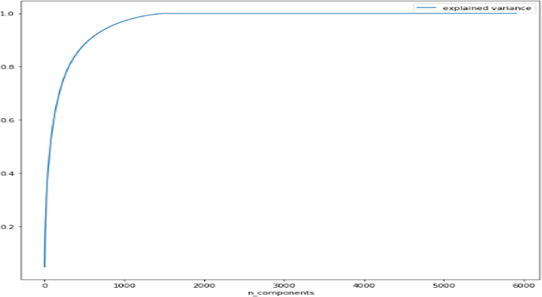
\includegraphics[width=0.8\textwidth]{media/ict/image6}
	\caption*{}
\end{figure}


{\bfseries 2 - сурет. Негізгі құрамдас әдісті пайдаланып өлшемділікті
азайту кезінде дисперсияны сақтау}

Жоғарыда келтірілген графикте көрсетілгендей, деректердің өлшемі 1285
белгіге дейін төмендеген жағдайда дисперсия 98,9 \% сақталады. Алайда,
жіктеу модельдерімен және деректер стандарттаушыларымен жүргізілген
тәжірибе көрсеткендей, бұл кішірейту конструктивті түрде жіктеудің
дәлдігіне ықпал етеді.

{\bfseries Материалдар мен әдістер.} Эксперимент жасау үшін деректерді
«Ақпараттық және есептеуіш технологиялар» инситутының зерттеушілерінің
базасынан алынды {[}9{]}. Берілген деректер, мәліметтер жиынтығы 0-19
сөйлеушінің 1285 аудио жазбасынан тұрды, олардың әрқайсысы 68-76
сөйлемнен тұратын жазбаны жазды. Қазақ тіліндегі әрбір аудиожазба орта
есеппен 5 секундқа созылатын сөз тіркесін білдіреді. Сөйлеушіні тану
үшін біз келесі деректер, мәліметтерді жинадық: сөйлеушінің аты,
сөйлеушінің жынысы, сөйлеушінің туған жері, сөйлеушінің туған жылы.
Төмендегі 1 кестеде сөйлеушінің мәліметтері көрсетілген.

{\bfseries 1 -- кесте. Сөйлеушінің мәліметтері}

% \begin{longtable}[]{@{}
%   >{\raggedright\arraybackslash}p{(\columnwidth - 12\tabcolsep) * \real{0.0943}}
%   >{\raggedright\arraybackslash}p{(\columnwidth - 12\tabcolsep) * \real{0.1578}}
%   >{\raggedright\arraybackslash}p{(\columnwidth - 12\tabcolsep) * \real{0.1068}}
%   >{\raggedright\arraybackslash}p{(\columnwidth - 12\tabcolsep) * \real{0.1961}}
%   >{\raggedright\arraybackslash}p{(\columnwidth - 12\tabcolsep) * \real{0.1237}}
%   >{\raggedright\arraybackslash}p{(\columnwidth - 12\tabcolsep) * \real{0.1540}}
%   >{\raggedright\arraybackslash}p{(\columnwidth - 12\tabcolsep) * \real{0.1673}}@{}}
% \toprule\noalign{}
% \begin{minipage}[b]{\linewidth}\raggedright
% ТАӘ
% \end{minipage} & \begin{minipage}[b]{\linewidth}\raggedright
% Тегі
% \end{minipage} & \begin{minipage}[b]{\linewidth}\raggedright
% Аты
% \end{minipage} & \begin{minipage}[b]{\linewidth}\raggedright
% Әкесінің аты
% \end{minipage} & \begin{minipage}[b]{\linewidth}\raggedright
% Жынысы
% \end{minipage} & \begin{minipage}[b]{\linewidth}\raggedright
% Туған жері
% \end{minipage} & \begin{minipage}[b]{\linewidth}\raggedright
% Туған жылы
% \end{minipage} \\
% \begin{minipage}[b]{\linewidth}\raggedright
% МЖА
% \end{minipage} & \begin{minipage}[b]{\linewidth}\raggedright
% Масимканова
% \end{minipage} & \begin{minipage}[b]{\linewidth}\raggedright
% Жазира
% \end{minipage} & \begin{minipage}[b]{\linewidth}\raggedright
% Ауезбеккызы
% \end{minipage} & \begin{minipage}[b]{\linewidth}\raggedright
% әйел
% \end{minipage} & \begin{minipage}[b]{\linewidth}\raggedright
% Алматы
% \end{minipage} & \begin{minipage}[b]{\linewidth}\raggedright
% 20.03.1982
% \end{minipage} \\
% \begin{minipage}[b]{\linewidth}\raggedright
% ИМТ
% \end{minipage} & \begin{minipage}[b]{\linewidth}\raggedright
% Искакова
% \end{minipage} & \begin{minipage}[b]{\linewidth}\raggedright
% Молдир
% \end{minipage} & \begin{minipage}[b]{\linewidth}\raggedright
% Тасболаткызы
% \end{minipage} & \begin{minipage}[b]{\linewidth}\raggedright
% әйел
% \end{minipage} & \begin{minipage}[b]{\linewidth}\raggedright
% Алматы
% \end{minipage} & \begin{minipage}[b]{\linewidth}\raggedright
% 01.01.1994
% \end{minipage} \\
% \begin{minipage}[b]{\linewidth}\raggedright
% ДАЖ
% \end{minipage} & \begin{minipage}[b]{\linewidth}\raggedright
% Дүйсенбаева
% \end{minipage} & \begin{minipage}[b]{\linewidth}\raggedright
% Айгерім
% \end{minipage} & \begin{minipage}[b]{\linewidth}\raggedright
% Жанболаткызы
% \end{minipage} & \begin{minipage}[b]{\linewidth}\raggedright
% әйел
% \end{minipage} & \begin{minipage}[b]{\linewidth}\raggedright
% Алматы
% \end{minipage} & \begin{minipage}[b]{\linewidth}\raggedright
% 15.05.1995
% \end{minipage} \\
% \begin{minipage}[b]{\linewidth}\raggedright
% ЖЕА
% \end{minipage} & \begin{minipage}[b]{\linewidth}\raggedright
% Жетписбаев
% \end{minipage} & \begin{minipage}[b]{\linewidth}\raggedright
% Ерлан
% \end{minipage} & \begin{minipage}[b]{\linewidth}\raggedright
% Алибекович
% \end{minipage} & \begin{minipage}[b]{\linewidth}\raggedright
% ер
% \end{minipage} & \begin{minipage}[b]{\linewidth}\raggedright
% Алматы
% \end{minipage} & \begin{minipage}[b]{\linewidth}\raggedright
% 23.05.1995
% \end{minipage} \\
% \begin{minipage}[b]{\linewidth}\raggedright
% ССМ
% \end{minipage} & \begin{minipage}[b]{\linewidth}\raggedright
% Самрат
% \end{minipage} & \begin{minipage}[b]{\linewidth}\raggedright
% Санжар
% \end{minipage} & \begin{minipage}[b]{\linewidth}\raggedright
% Мұхаметқалиулы
% \end{minipage} & \begin{minipage}[b]{\linewidth}\raggedright
% ер
% \end{minipage} & \begin{minipage}[b]{\linewidth}\raggedright
% Алматы
% \end{minipage} & \begin{minipage}[b]{\linewidth}\raggedright
% 12.07.1996
% \end{minipage} \\
% \midrule\noalign{}
% \endhead
% \bottomrule\noalign{}
% \endlastfoot
% \end{longtable}

\emph{Жіктеу алгоритмдері}

Сөйлеушіні анықтау тану мәселесін шешуде төмендегідей жіктеу
алгоритмдерін қарастырдық:

\emph{MLP Classifier алгоритмі}

MLP көп қабатты перцептрон -
\((Y) = T_{n}:{\ \ T}_{n} \rightarrow T^{0}\) функциясын аудио деректер
сериясында оқыту арқылы зерттейтін басқарылатын оқыту алгоритмі, мұндағы
n - енгізу үшін өлшемдер саны, а\textsubscript{0}-шығару үшін өлшемдер
саны. \(Y = y_{1},y_{2},\ldots,y_{n}\) функцияларының жиынтығын ескере
отырып ` \(y_{n}\)' ол кез-келген классификация үшін сызықтық емес
функциялардың жуықтауын зерттей алады. 3-ші суретте MLP архитектурасы
көрсетілген.

\begin{figure}[H]
	\centering
	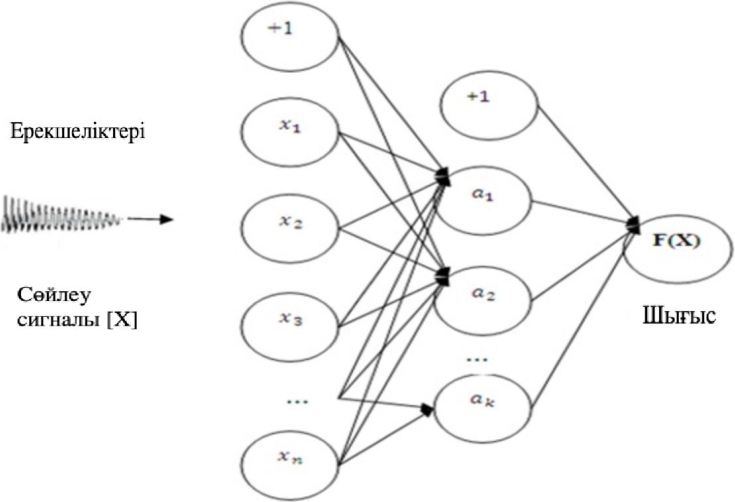
\includegraphics[width=0.8\textwidth]{media/ict/image7}
	\caption*{}
\end{figure}


{\bfseries \hl{3}} -- {\bfseries \hl{сурет}}. {\bfseries \hl{MLP архитектурасы}}

Кіріс қабаты кіріс функцияларын білдіретін
\hl{}\(x_{1},\ x_{2},\ ...,x_{n\ }\ \)тұрады. Шығыс қабаты соңғы жасырын
қабаттан мәндерді алады және оларды шығару мәндеріне түрлендіреді.

\emph{Extra-Trees алгортимі}

Extra-Trees алгоритмі жаңартылмайтын шешімдер немесе регрессиялар
ансамблін жасайды. Қадамға негізделген ансамбльдің басқа әдістері
алгоритмнің екі негізгі айырмашылығы-ол кездейсоқ түрде кесу нүктелерін
таңдап, түйіндерді сындырады және қадамдарды ұлғайту үшін бүкіл оқу
үлгісін пайдаланады {[}10{]}.

\emph{Trees\_node(M)}

Тұрақты оқыту жиынтығы N түйініне сәйкес келіп кіріс синалын айналады.

шығыс синалы ретінде {[}\(d\) \textless{} \(d_{c}\){]} аламыз

-- оқытуда \emph{Tree(S.)} ақиқат болған жаңдайда ешнәрсе қайтарылмайды

-- ондай жағдайда тұрақты емес барлық (S) атрибуттарының топтарының
ішіндегі \{\(d_{1}\),...\({,d}_{K}\)\} атрибуттарын тұрақты түрде
таңдаймыз;

-- осы K қадамдарды \{g\textsubscript{1},...,g\textsubscript{K} \}
таңдап, мұндағы g\textsubscript{i} = \emph{Random\_split.}(G,
d\textsubscript{i}), ∀ i = 1,..., K.;

--g\textsubscript{∗} сегменттерінде Score(g\textsubscript{∗}, G.) =
max\textsubscript{i=1,...,K} Score(g\textsubscript{i}, G.) деп
келтіреміз.

\emph{Random\_split.(S,} \(a\)\emph{)}

G ішкі жиыны және d атрибуты кірісі.

-- \(d_{\max}^{G}\) және \(d_{\min}^{G}\) минималды мәнді, максималды
мәнін G-ге біріктіреді;

\emph{Tree(S.)}

G ішкі жиынның кірісі

\(d\) логикалық мәні шығысы

-- егерде \textbar{} G \textbar{} \textless{} n\textsubscript{min} болса
қайтару ақиқатты көрсетеді;

-- егер барлық G атрибуттары тұрақты болса, біз TRUE (ақиқат)мәнін
қайтарамыз;

-- егер G шығысы тұрақты болса, біз true (ақиқат)қайтарамыз;

-- болмаған жағдайда біз false (жалған) мәнін қайтарамыз.

Оның екі параметрі бар: K әр түйін үшін кездейсоқ таңдалған атрибуттар
саны және n\textsubscript{min} түйінді бөлу үшін ең кіші үлгінің өлшемі.
Ол ансамбль моделін құру үшін бастапқы оқыту моделімен бірнеше рет
қолданылады {[}11{]}.

\emph{SVC алгоритмі}

Сызықтық бөлінетін екілік жіктеу мәселесін шешу үшін SVC пайдалану үшін
бізге қажет:

\begin{itemize}
\item
  \emph{J-}ді құруда{\bfseries ,} мұндағы
  \(J_{ij} = z_{i}z_{j}y_{i} \bullet y_{j}\)
\item
  σ --ны табу;
\item
  \(\sum_{i = 1}^{M}{}{\sigma\ }_{i} - \frac{1}{2}{\sigma\ }^{T}J\sigma\ \)
\item
  \({\sigma\ }_{i} \geq 0\ \ \ \ \ \ \forall_{i}\ және\ \sum_{i = 1}^{M}{}{\sigma\ }_{i}z_{i} = 0\ \)осы
  шектеу аймақтарын ескере қарап, мейілінше жоғарылату;
\item
  QN шешімді қолдану болып табылады;
\item
  \(v = \sum_{i = 1}^{M}{}{\sigma\ }_{i}z_{i}y_{i}\) есептеу;
\item
  \({\sigma\ }_{i} > 0\ \ \ \ \ \ \)индекстерін есептеп, \emph{l} тірек
  әрбір векторының санын анықтау;
\item
  \(a = \frac{1}{M_{s}}\sum_{l \in L}^{}{}({\sigma\ }_{m}z_{m}y_{m} \bullet y_{L}\)
  есептеу керек;
\item
  \(y^{'}\ \)кез-келген нүктесі \(z^{'} = sgn(v \bullet y^{'} + a\)
  есептеу тәсілімен жіктеуге болады.
\end{itemize}

\emph{Gaussian NB алгоритмі}

Осы Naive Bayes - \(y_{1},\ y_{2},\ ...,y_{n\ }\) тізбегіндегі
көбейтіндісіне с пропорционал \(А_{k}\)класының ішінде жататын
\(m + 1\ \)деректер нүктесінің нақты ықтималдығын береді. \(m\)
алдыңғы\(\ \sigma\left( A_{k} \right) -\)класы мен
\(\sigma\left( А_{a} \right)\prod_{i = 1}^{m}{}\sigma\left( A_{k} \right)\ \)белгілерінің
арасындағы шартты ықтималдығы болып табылады {[}12{]}.

\(\sigma(A_{a}\))\(\prod_{i = 1}^{m}{}\sigma\left( A_{a} \right) > \sigma(A_{b})\prod_{i = 1}^{m}{}\sigma(y_{i}|A_{b})\)

\[\sigma\left( y_{1},\ldots,y_{n} \right) > \sigma(A_{b}|y_{1},\ldots,\ y_{n})\]

Осылайша, \(y_{1},\ y_{2},\ ...,y_{n\ }\ \) мәліметтер нүктесіне кластың
осы ең ықтимал нақты тағайындалуы \(а = 1,\ldots,А\) үшін
\(\sigma\left( А_{a} \right)\prod_{i = 1}^{m}{}\ \sigma\left( A_{k} \right)\ \)есептеудің
мәні макисмум болып табылатын \(А_{k}\ \)класындағы
\(y_{1},\ y_{2},\ ...,y_{n\ }\ \)есептеу ықтималдығы.

\emph{KNN алгоритмі}

KNN алгоритмі сұрау көрінісі мен мәліметтер жиынтығындағы көрініс
жиынтығы арасындағы ара қашықтықты өлшейді.

Тестілеу модельдеу нысандарының әрқайсысын жіктеу үшін келесі
әрекеттерді жүйелі түрде орындау қажет:

- оқыту моделінің әрбір нысанына дейінгі ара қашықтықты есептеу керек;

- K-ны оқыту моделінің нысанын таңдау керек;

- К классификацияланған объектінің класы жақын көршілер арасында ең көп
таралған класс болып табылады.

Жоғарыдағы ұсынылған алгоритмдер тұлғаны сәйкестендіру, сөйлеушіні тану
мәселесіне қолданылып, салыстырмалы талдау жүргізілді. Салыстырмалы.
талдаулар мен эксперименттер олардың ең жақсы екенін көрсетеді.
Нәтижелерінде тірек векторлық машиналар мен көп қабатты перцептронды
қолдану арқылы алынды. 4-ші суретте осы мәліметтер жиынының жіктеу
дәлдігі көрсетілген.

\begin{figure}[H]
	\centering
	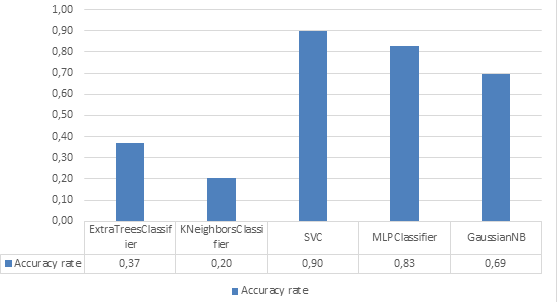
\includegraphics[width=0.8\textwidth]{media/ict/image8}
	\caption*{}
\end{figure}


{\bfseries 4 -- сурет. Деректер жиынының жітеу дәлдігі}

4-ші суреттен көрініп тұрғандай тірек векторлық машина мен көпқабатты
перцептрон ең жақсы нәтиже көрсетті -- сәйкесінше 0,90 және 0,83.

Нәтижелерді жақсарту үшін біз әртүрлі әдістерді қолданып масштабтау
жасап, нәтижелердің өзгергені байқалды. 5 -- суретте әртүрлі әдістерді
қолдану арқылы деректерді масштабтау кезіндегі жіктеу дәлдігі
көрсетілген.

\begin{figure}[H]
	\centering
	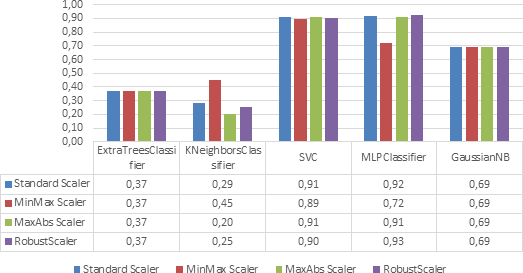
\includegraphics[width=0.8\textwidth]{media/ict/image9}
	\caption*{}
\end{figure}


{\bfseries 5 -- сурет. Әртүрлі әдістерді қолдану арқылы деректерді
масштабтау кезіндегі жіктеу дәлдігі}

Көпқабатты перцептрон сенімді Robust scaler әдісін қолданып масштабтаған
кезде ең жоғары дәлдікке 0,93 жетті, ал тірек векторлық машиналар
дәлдігі азая бастады, бірақ Standard scaler және MaxAb Scaler әдісімен
масштабтау кезінде дәлдік нәтижелері 0,90-нан 0,91-ге дейін жақсарды.

Сөйлеу нысандарының өлшемділігін 1390-ға дейін азайту үшін негізгі
құрамдас талдауды пайдалансаңыз, жіктеу дәлдігі 2-кестеде көрсетілгендей
өзгереді.

{\bfseries 2 - кесте. Өлшемді азайту арқылы деректер бойынша жіктеу
дәлдігі}

\begin{figure}[H]
	\centering
	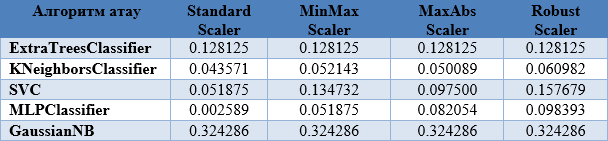
\includegraphics[width=0.8\textwidth]{media/ict/image10}
	\caption*{}
\end{figure}


Салыстырмалы талдаудың мақсаты жеке сөйлеушіні тану мәселесіне жіктеу
алгоритмінің әсер ету дәрежесін анықтау, сонымен қатар SVC және MLP
жіктеуіш алгоритмдерін салыстырмалы бағалау болды. Дауыс деректерінің
үлгілерін оқыту бойынша жүргізілген эксперименттер осы алгоритмдердің
келешегі туралы айтуға мүмкіндік беретін нәтижелерді көрсетеді. Алынған
мәліметтер 6 және 7-суреттерде берілген.

\begin{figure}[H]
	\centering
	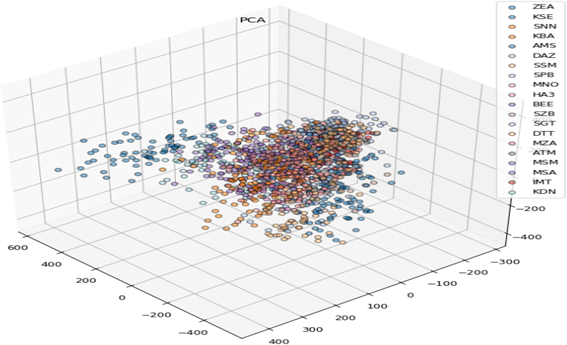
\includegraphics[width=0.8\textwidth]{media/ict/image11}
	\caption*{}
\end{figure}


{\bfseries 6 -- сурет. Дыбыстық деректердің, сөйлеу белгілерінің үш өлшемді
көрінісі}

\begin{figure}[H]
	\centering
	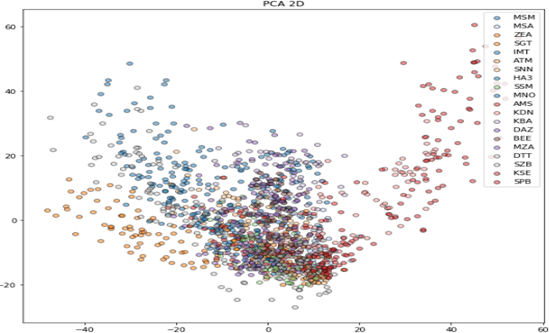
\includegraphics[width=0.8\textwidth]{media/ict/image12}
	\caption*{}
\end{figure}


{\bfseries 7 -- сурет. Дыбыстық деректердің, сөйлеу белгілерінің екі
өлшемді көрінісі}

Әртүрлі әдістерді қолдану арқылы деректерді, масштабтау кезіндегі жіктеу
нәтижелері алдын ала экспериментте алынған нәтижелерден айтарлықтай
ерекшеленетіні анықталды.

{\bfseries Қортынды.} Бұл мақалада біз бірнеше жіктеу алгоритмдерін және
сөйлеуді алдын ала өңдеу мәселесін қарастырдық. Тәжірибе нәтижелерін
талдау негізінде Robust scaler әдісімен масштабтау үшін дәлдігі 0,93
көпқабатты перцептрон ұсынылады, ал сөйлеу сигналын көпқабатты
перцептрон көмегімен жіктеуге болатындығы анықталды. Содан кейін алынған
деректерге сүйене отырып, сөйлеушіні тану үдерісін анықтадық.

Әрі қарайғы зерттеу барысында біз алынған мәліметтердің шынайылығын
тексеру мәселесін шешеміз деп үміттенеміз.

{\bfseries Әдебиеттер}

\begin{enumerate}
\def\labelenumi{\arabic{enumi}.}
\item
  Matejka, P.; Zhang, L.; Ng, T.; Glembek, O.; Ma, J.; Zhang, B.;
  Mallidi, S.H. Neural Network Bottleneck Features for Language
  Identification // In Proceedings of the Speaker and Language
  Recognition Workshop (Odyssey 2014). - Joensuu, Finland, 16--19 June
  2014. -P. 299--304. DOI: 10.21437/Odyssey.2014-45
\item
  Pliakos K., Geurts P., Vens C. Global multi-output decision trees for
  interaction prediction // Machine Learning. - 2018.- P. 1--25.
  DOI:10.1007/s10994-018-5700-x
\end{enumerate}

3.\href{https://www.scopus.com/authid/detail.uri?authorId=55967630400}{Mamyrbayev,
O.},~\href{https://www.scopus.com/authid/detail.uri?authorId=57200275502}{Toleu,
A.},~\href{https://www.scopus.com/authid/detail.uri?authorId=57200276217}{Tolegen,
G.},~\href{https://www.scopus.com/authid/detail.uri?authorId=57202316868}{Mekebayev,
N.}, Neural architectures for gender detection and speaker
identification//Cogent Engineering.- 2020.-Vol.7(1).

\href{https://doi.org/10.1080/23311916.2020.1727168}{DOI
10.1080/23311916.2020.1727168}

\begin{enumerate}
\def\labelenumi{\arabic{enumi}.}
\setcounter{enumi}{2}
\item
  R. Wolff, " MonkeyLearn Blog," 5 Types of Classification Algorithms
  inMachine Learning, 26 August 2020.
\item
  \href{https://www.scopus.com/authid/detail.uri?authorId=56153126500}{Kalimoldayev,
  M.N.},~\href{https://www.scopus.com/authid/detail.uri?authorId=55967630400}{Mamyrbayev,
  O.Zh.},~\href{https://www.scopus.com/authid/detail.uri?authorId=57208346238}{Kydyrbekova,
  A.S.},~\href{https://www.scopus.com/authid/detail.uri?authorId=57202316868}{Mekebayev,
  N.O.} Voice verification and identification using i-vector
  representation // International Journal of Mathematics and Physics.
  -2019. -Vol. 10(1).- P. 66--74/ DOI 10.26577/ijmph-2019-i1-9
\item
  Hazmoune S, Bougamouza F, Mazouzi S. A new hybrid framework based on
  hidden Markov models and K-nearest neighbors for speech recognition //
  International Journal of Speech Technology.- 2018.-Vol. 21(3). -P.
  689-704. DOI 10.1007/s10772-018-9535-4
\item
  Mamyrbayev O, Turdalyuly M, Mekebayev N, Alimhan K, Kydyrbekova A,
  Turdalykyzy T. Automatic recognition of Kazakh speech using deep
  neural networks // ,In: Asian Conference on Intelligent Information
  and Database Systems. -2019. -P. 465-474.
  \hl{DOI\href{http://dx.doi.org/10.1007/978-3-030-14802-7_40}{10.1007/978-3-030-14802-7\_40}}
\item
  Hinton, G., Deng, L., Yu, D., Dahl, G. E., Mohamed, A.-r., Jaitly, N.,
  Senior, A., Vanhoucke, V., Nguyen, P., Sainath, T. N., \& Kingsbury,
  B. Deep Neural Networks for Acoustic Modeling in Speech Recognition:
  The Shared Views of Four Research Groups // IEEE Signal Processing
  Magazine. -2012. -Vol. 29(6). -P. 82-97.
  \href{https://doi.org/10.1109/MSP.2012.2205597}{DOI
  10.1109/MSP.2012.2205597}
\item
  \href{https://www.scopus.com/authid/detail.uri?authorId=56153126500}{Kalimoldayev,
  M.},~\href{https://www.scopus.com/authid/detail.uri?authorId=55967630400}{Mamyrbayev,
  O.},~\href{https://www.scopus.com/authid/detail.uri?authorId=57202316868}{Mekebayev,
  N.},~\href{https://www.scopus.com/authid/detail.uri?authorId=57208346238}{Kydyrbekova,
  A.} Algorithms for detection gender using neural networks //
  \hl{International Journal of Circuits, Systems and Signal
  Processing\emph{. -}2020. -Vol. 14}.- P. \hl{154--159. DOI
  \href{https://doi.org/10.46300/9106.2020.14.24}{10.46300/9106.2020.14.24}}
\item
  Zhan C, Li W, Ogunbona P. Face recognition from single sample based on
  human face perception // In: International Conference Image and Vision
  Computing New Zealand. - 2009. -P. 56-61.
  \href{https://doi.org/10.1109/IVCNZ.2009.5378397}{DOI10.1109/IVCNZ.2009.5378397}
\item
  R. Praba, G. Darshan, K. T. Roshanraj. and P. B. Surya Prakash.
  StudyOn Machine Learning Algorithms//International Journal of
  ScientificResearch in Computer Science, Engineering and Information
  Technology.-2021.-Vol.7(4)- P.67-72, 2021.
\end{enumerate}

11.V. B. Vaghela, B. M. Jadav. Analysis of various sentiment
classification techniques.// Int. J. Comput. Appl..-2016.- Vol. 140
(3).- P. 22-27.\href{https://doi.org/10.5120/ijca2016909259}{DOI
10.5120/ijca2016909259}.

\emph{{\bfseries Авторлар туралы мәліметтер}}

Мекебаев Н.О. - PhD, Қазақ ұлттық қыздар педагогикалық университетінің
қауымдастрылған профессор м.а., Алматы, Қазақстан, e-mail:
\emph{\href{mailto:nurbapa@gmail.com}{\nolinkurl{nurbapa@gmail.com}};}

\hl{Даркенбаев Д.К.}- \hl{PhD, әл-Фараби атындағы Қазақ ұлттық
университетінің доцент м.а., Алматы, Қазақстан, e-mail:
\href{mailto:dauren.kadyrovich@gmail.com}{\nolinkurl{dauren.kadyrovich@gmail.com}};}

\hl{Модовов Н.А.- магистр,} Қазақ ұлттық қыздар педагогикалық
университетінің аға оқытушысы, Алматы, Қазақстан, e-mail:
\href{mailto:modovov@mail.ru}{\nolinkurl{modovov@mail.ru}};

.Орынтаева Ж.А -- магистр, Қазақ ұлттық қыздар педагогикалық
университетінің аға оқытушысы, Алматы, Қазақстан, e-mail:
\href{mailto:Zannaoryntaeva0@gmail.ru}{\nolinkurl{Zannaoryntaeva0@gmail.ru}}

\emph{{\bfseries Information about the authors}}

Mekebayev N.-PhD, \hl{Acting Associate Professor} Kazakh National
Women' s Pedagogical University, Almaty, Kazakhstan,
e-mail:
\emph{\href{mailto:nurbapa@gmail.com}{\nolinkurl{nurbapa@gmail.com}};}

Darkenbayev D.- PhD, \hl{Acting Associate Professor} Al-Farabi Kazakh
National University, Almaty, Kazakhstan e-mail:
\href{mailto:dauren.kadyrovich@gmail.com}{\nolinkurl{dauren.kadyrovich@gmail.com}};

Modovov N.- master, Kazakh National Women' s Pedagogical
University, Almaty, Kazakhstan, e-mail:
\href{mailto:modovov@mail.ru}{\nolinkurl{modovov@mail.ru}};

Oryntaeva Zh.- master, Kazakh National Women' s
Pedagogical University, Almaty, Kazakhstan, e-mail:
\href{mailto:Zannaoryntaeva0@gmail.ru}{\nolinkurl{Zannaoryntaeva0@gmail.ru}}

ГРНТИ 28.23.02

{\bfseries МЕТОДЫ КОНТРОЛЯ УТОМЛЯЕМОСТИ ВОДИТЕЛЕЙ С ИСПОЛЬЗОВАНИЕМ
ТЕХНОЛОГИЙ МАШИННОГО ОБУЧЕНИЯ}

{\bfseries \textsuperscript{1}А.Ж.Танирбергенов}
\begin{figure}[H]
	\centering
	
\includegraphics[width=0.8\textwidth]{media/ict/image1}
	\caption*{}
\end{figure}

\textsuperscript{1}С.К.Серикбаева\textsuperscript{\envelope }}
\begin{figure}[H]
	\centering
	
\includegraphics[width=0.8\textwidth]{media/ict/image1}
	\caption*{}
\end{figure}

\textsuperscript{2}Б.Тасуов}
\begin{figure}[H]
	\centering
	
\includegraphics[width=0.8\textwidth]{media/ict/image1}
	\caption*{}
\end{figure}

\textsuperscript{3}Г.Ш.Мусагулова}
\begin{figure}[H]
	\centering
	
\includegraphics[width=0.8\textwidth]{media/ict/image1}
	\caption*{}
\end{figure}

{\bfseries ,}

{\bfseries \textsuperscript{3}Л.Ақзуллақызы}
\begin{figure}[H]
	\centering
	
\includegraphics[width=0.8\textwidth]{media/ict/image1}
	\caption*{}
\end{figure}

\begin{figure}[H]
	\centering
	
\includegraphics[width=0.8\textwidth]{media/ict/image1}
	\caption*{}
\end{figure}


\emph{\textsuperscript{1}Евразийский национальный университет имени
Л.Н.Гумилева, Астана, Казахстан,}

\emph{\textsuperscript{2}Таразский региональный университет им.М. Х.
Дулати, Тараз, Казахстан,}

\emph{\textsuperscript{3}Кызылординский университет имени Коркыт Ата,
Кызылорда, Казахстан}

{\bfseries \textsuperscript{\envelope }}\emph{Корреспондент-автор:
\href{mailto:inf_8585@mail.ru}{\nolinkurl{inf\_8585@mail.ru}}}

В статье рассматриваются методы разработки интеллектуальной системы
мониторинга состояния усталости водителей с применением технологий
машинного обучения. Усталость водителя является одной из ведущих причин
дорожно-транспортных происшествий, особенно на длительных маршрутах и
при ночных сменах. Предложенная модель на основе коэффициента пропорции
глаз (EAR) и классификатора с использованием метода опорных векторов
(SVM) обеспечивает эффективное детектирование морганий и других
признаков усталости в режиме реального времени. Особое внимание уделено
устойчивости модели к изменениям условий освещения и ориентации головы,
что повышает надежность системы в сложных эксплуатационных условиях.
Особенностью разработанной системы является устойчивость к изменяющимся
условиям, включая изменения освещения и углов наклона головы водителя,
что улучшает надежность модели в сложных эксплуатационных условиях. В
статье отмечается, что применение данной технологии возможно в различных
интеллектуальных транспортных системах, поскольку тестирование показало
высокие показатели точности и минимальное количество ложных
срабатываний.

В результате тестирования предложенной системы были получены высокие
показатели точности, что делает ее подходящей для использования в
интеллектуальных транспортных системах. Ключевым преимуществом
предлагаемой системы является её устойчивость к изменениям условий
освещения и ориентации головы водителя, что значительно повышает
точность и надежность работы системы в сложных эксплуатационных
условиях.

{\bfseries Ключевые слова:} усталость водителя, мониторинг состояния,
машинное обучение, детектирование морганий, интеллектуальная система,
коэффициент пропорции глаз, SVM, компьютерное зрение.

{\bfseries МАШИНАЛЫҚ ОҚЫТУ ТЕХНОЛОГИЯЛАРЫН ҚОЛДАНА ОТЫРЫП ЖҮРГІЗУШІЛЕРДІҢ
ШАРШАҒЫШТЫҒЫН БАҚЫЛАУ ӘДІСТЕРІ}

{\bfseries \textsuperscript{1}А.Ж. Танирбергенов, \textsuperscript{1}С.К.
Серикбаева\textsuperscript{\envelope }, \textsuperscript{2}Б. Тасуов,
\textsuperscript{3}Г.Ш. Мусагулова,}

{\bfseries \textsuperscript{3}Л. Ақзуллақызы,
\textsuperscript{3}Б.К.Жарменова}

\emph{\textsuperscript{1}Л.Н.Гумилев атындағы Еуразия ұлттық
университеті, Астана қ., Қазақстан,}

\emph{\textsuperscript{2}М.Х.Дулати атындағы Тараз өңірлік университеті,
Тараз қ., Қазақстан,}

\emph{\textsuperscript{3}Қорқыт Ата атындағы Қызылорда университеті,
Қызылорда қ., Қазақстан,}

\emph{e-mail: inf\_8585@mail.ru}

Мақалада машиналық оқыту технологияларын қолдана отырып, жүргізушілердің
шаршау жай-күйін мониторингілеудің зияткерлік жүйесін әзірлеу әдістері
қарастырылады. Жүргізушінің шаршауы жол-көлік оқиғаларының, әсіресе ұзақ
бағыттар мен түнгі ауысымдар кезіндегі басты себептерінің бірі болып
табылады. Ұсынылған модель көз пропорциясының коэффициенті (EAR) және
тірек векторлары (SVM) әдісін пайдалана отырып жіктеуіш негізінде нақты
уақыт режимінде морганиялар мен шаршаудың басқа да белгілерін тиімді
анықтауды қамтамасыз етеді. Үлгінің жарықтандыру жағдайларының өзгеруіне
және бастың бағдарына орнықтылығына ерекше назар аударылады, бұл күрделі
пайдалану жағдайларында жүйенің сенімділігін арттырады. Әзірленген
жүйенің ерекшелігі күрделі пайдалану жағдайларында модельдің
сенімділігін жақсартатын жарықтандыру мен жүргізуші басының көлбеу
бұрыштарының өзгеруін қоса алғанда, өзгермелі жағдайларға төзімділік
болып табылады. Мақалада аталған технологияны әртүрлі зияткерлік көлік
жүйелерінде қолдануға болатындығы атап өтілген, себебі тестілеу жоғары
дәлдік көрсеткіштерін және жалған іске қосылулардың ең аз санын
көрсетті.

Ұсынылған жүйені тестілеу нәтижесінде жоғары дәлдік көрсеткіштері
алынды, бұл оны зияткерлік көлік жүйелерінде пайдалану үшін қолайлы
етеді. Ұсынылып отырған жүйенің негізгі артықшылығы оның жарықтандыру
жағдайларының өзгеруіне және жүргізуші басының бағдарына төзімділігі
болып табылады, бұл күрделі пайдалану жағдайларында жүйенің жұмысының
дәлдігі мен сенімділігін едәуір арттырады.

{\bfseries Түйін сөздер:} жүргізушінің шаршауы, жағдайды бақылау, Машиналық
оқыту, жыпылықтауды анықтау, интеллектуалды жүйе, көздің пропорция
коэффициенті, SVM, компьютерлік көру.

{\bfseries METHODS OF DRIVER FATIGUE CONTROL USING MACHINE LEARNING
TECHNOLOGIES}

{\bfseries \textsuperscript{1}А. Tanirbergenov, \textsuperscript{1}S.
Serikbayeva\textsuperscript{\envelope }, \textsuperscript{2}B. Tassuov,
\textsuperscript{3}G. Mussagulova,}

{\bfseries \textsuperscript{3}L. Akzullakyzy, \textsuperscript{3}B.
Zharmenova}

\emph{\textsuperscript{1}L.N. Gumilyov Eurasian National University,
Astana, Kazakhstan,}

\emph{\textsuperscript{2}Taraz Regional University named after M.Kh.
Dulaty, Taraz, Kazakhstan,}

\emph{\textsuperscript{3}Korkyt Ata Kyzylorda University, Kyzylorda,
Kazakhstan,}

\emph{e-mail:
\href{mailto:inf_8585@mail.ru}{\nolinkurl{inf\_8585@mail.ru}}}

The article discusses methods for developing an intelligent driver
fatigue monitoring system using machine learning technologies. Driver
fatigue is one of the leading causes of road accidents, especially on
long routes and night shifts. The proposed eye proportion ratio (EAR)
and support vector classifier (SVM) model provides effective real-time
detection of blinks and other signs of fatigue. Particular attention is
paid to the model' s resistance to changes in lighting
conditions and head orientation, which increases the reliability of the
system in difficult operating conditions. A feature of the developed
system is resistance to changing conditions, including changes in
lighting and tilt angles of the driver' s head, which
improves the reliability of the model in difficult operating conditions.
The article notes that the application of this technology is possible in
various intelligent transport systems, since testing has shown high
accuracy rates and a minimum number of false positives.

As a result of testing the proposed system, high accuracy indicators
were obtained, which makes it suitable for use in intelligent transport
systems. The key advantage of the proposed system is its resistance to
changes in lighting conditions and orientation of the
driver' s head, which significantly increases the
accuracy and reliability of the system in difficult operating
conditions.

{\bfseries Keywords:} driver fatigue, condition monitoring, machine
learning, blink detection, intelligent system, eye proportion
coefficient, SVM, computer vision.

{\bfseries Введение} Методы интеллектуальной системы контроля усталостного
состояния водителей с использованием технологий машинного обучения"
представляет собой обзор современных подходов и технологий, направленных
на обеспечение безопасности дорожного движения за счет раннего выявления
усталости водителей.

Усталость за рулем является широко распространенным явлением,
возникающим в результате длительного вождения или недостатка сна. Это
серьезная потенциальная угроза для безопасности дорожного движения, о
чем свидетельствует статистика: в США ежегодно происходит около 100 000
дорожно-транспортных происшествий, связанных с усталостью водителей, в
результате которых 400 000 человек получают ранения, а 1550 теряют
жизнь. В связи с этим исследования по обнаружению усталости во время
вождения становятся актуальной научно-практической задачей во всем мире.

Для повышения безопасности на дорогах необходимо регулярно проверять
состояние водителей и оценивать их манеру вождения. Прогнозирование
поведения водителя представляет собой важную часть интеллектуальных
транспортных систем и играет ключевую роль в их разработке. В ходе ряда
исследований ведущими производителями автомобилей были разработаны и
успешно внедрены несколько методик контроля состояния водителей, включая
определение сонливости и рассеянности.

В этом контексте используются различные аппаратные компоненты, такие как
мобильные камеры и датчики. Информация, полученная с гироскопа,
акселерометра и глобальной системы позиционирования (GPS), собирается
для выявления критических закономерностей, связанных с поведением
водителя. С развитием искусственного интеллекта, Интернета вещей и
технологий компьютерного зрения появляются более усовершенствованные
системы мониторинга состояния водителя и определения степени усталости,
что делает автомобили более «умными» и способными предотвращать аварии
на дорогах. Основными компонентами таких систем являются
микроконтроллеры и различные датчики, включая датчики моргания глаз,
ударов, датчики определения алкоголя и уровня топлива. API GPS и Google
Maps используются для отслеживания местоположения автомобиля. Такие
интегрированные системы могут значительно повысить безопасность
дорожного движения и снизить количество ДТП, связанных с усталостью
водителей.

{\bfseries Обзор литературы.} Проблема утомляемости является одним из
ключевых факторов дорожно-транспортных происшествий, особенно на
длительных маршрутах и при ночных сменах. Водитель, находящийся в
состоянии усталости, теряет концентрацию, замедляется реакция, и
возрастает риск аварийных ситуаций, что ставит под угрозу не только его
собственную жизнь, но и жизнь других участников дорожного движения.

С развитием современных технологий и доступностью датчиков различных
типов появилась возможность автоматизировать процесс мониторинга
состояния водителей. Системы контроля усталости, использующие методы
машинного обучения, способны анализировать множество факторов в реальном
времени, включая поведенческие, физиологические и внешние параметры,
такие как движения глаз, положение головы, частоту морганий и другие.
Использование алгоритмов искусственного интеллекта позволяет не только
повысить точность диагностики усталости, но и адаптировать систему под
особенности каждого водителя, что способствует снижению ложных
срабатываний и повышению общей эффективности системы. На данный момент
на рынке уже существуют различные системы мониторинга усталости, но
большинство из них сталкиваются с проблемами низкой точности при сложных
внешних условиях, а также высокой стоимостью оборудования, что
ограничивает их повсеместное использование. Более того, многие решения
основаны на ограниченном наборе данных, что снижает их универсальность и
адаптивность к различным сценариям эксплуатации. Именно в этом контексте
возникает необходимость разработки новых подходов, сочетающих в себе
высокую точность, устойчивость к внешним факторам и доступность. Одним
из наиболее перспективных решений является применение глубоких нейронных
сетей и методов машинного обучения для анализа данных, поступающих с
различных сенсоров в транспортных средствах. Такие системы способны в
режиме реального времени предсказывать наступление усталости водителя,
что дает возможность вовремя предупреждать его о необходимости отдыха
или смены водителя. В этой связи стоит выделить роль моделей
компьютерного зрения, анализа биометрических данных, а также интеграции
с системами предупреждения и автоматического контроля транспортных
средств.

В статье {[}1{]} рассматриваются перспективы и возможности использования
интеллектуальных систем мониторинга усталости водителя для повышения
безопасности на дорогах. Отмечается, что благодаря развитию современных
технологий, данные системы способствуют значительному снижению
количества дорожно-транспортных происшествий. Проведён анализ
показывает, что интеллектуальные системы способны на ранних этапах
выявлять отклонения в поведении водителя, что позволяет оперативно
генерировать предупреждающие сигналы и оповещения. Сделан вывод, что
наибольшая эффективность в контроле состояния водителя достигается за
счёт комбинирования различных методов и приёмов интеллектуального
анализа данных.

В статье {[}2{]} рассматриваются актуальные вопросы, касающиеся контроля
состояния водителя автомобиля. Подчёркивается, что в настоящее время
разработан широкий спектр методов, которые можно разделить на
физиологические, поведенческие и автомобильные. Системы, основанные на
физиологических и поведенческих данных, демонстрируют высокий уровень
точности и надежности в режиме реального времени. Выявлено, что
эффективность описанных методов может быть значительно повышена с
помощью технологий интеллектуального анализа, таких как нейронные сети и
компьютерное зрение. Сделан вывод о том, что интеллектуальные технологии
позволяют эффективно управлять рисками, связанными с усталостью и
отвлечением внимания водителя.

В статье {[}3{]} проведён анализ методов детектирования утомления
водителей, используемых в современной литературе. Обсуждается широкий
спектр методов, применяемых для оценки функционального состояния
человека, которое представляет собой интегральный комплекс характеристик
функций и качеств, определяющих успешность выполнения различных видов
деятельности. Функциональное состояние организма напрямую влияет на
физическое и психическое состояние человека, а также на результаты его
труда, обучения и творчества. Оценка динамического поведения водителя в
последние годы становится одним из самых актуальных направлений
исследований. Динамическая оценка включает продолжительный мониторинг,
который позволяет определять функциональные состояния.

В работе {[}4{]} рассматривается подход к распознаванию стиля вождения
водителя транспортного средства с использованием сенсоров смартфона.
Основное внимание уделено методам анализа данных, полученных с
акселерометра, гироскопа и GPS-датчика мобильного устройства, для
выявления характерных особенностей поведения водителя. Предложенный
подход позволяет классифицировать стили вождения, такие как агрессивный,
умеренный и спокойный, что может быть полезным для повышения
безопасности дорожного движения, оценки навыков водителя и разработки
персонализированных рекомендаций.

В работе {[}5{]} рассматриваются возможности прогнозирования аварийности
водителей на основе анализа их поведенческих характеристик и факторов,
влияющих на вероятность совершения дорожно-транспортных происшествий. В
исследовании акцентируется внимание на таких аспектах, как стаж
вождения, индивидуальный стиль управления транспортным средством и
склонность к рисковому поведению. Применение статистических методов
анализа и современных технологий, включая телематические устройства и
сенсоры, позволяет выявлять потенциально опасные модели поведения
водителей, что может быть полезно для повышения уровня безопасности
дорожного движения и разработки превентивных мер.

В работе {[}6{]} рассматриваются методы и средства контроля состояния
водителя автомобиля, направленные на повышение безопасности дорожного
движения. Основное внимание уделено современным технологиям, позволяющим
мониторить физиологические и поведенческие параметры водителя, такие как
частота сердечных сокращений, электрическая активность кожи, движения
глаз и головы. Обсуждаются возможности использования систем
видеонаблюдения, датчиков и интеллектуальных алгоритмов для
своевременного выявления признаков утомления, снижения концентрации и
других факторов, влияющих на управление транспортным средством. Также
анализируются перспективы интеграции таких систем в современные
автомобили.

Авторы {[}7{]} рассматривают различные подходы к обнаружению сонливости
водителей, включая анализ физиологических сигналов, характеристик лица и
стиля вождения. Обсуждаются преимущества и ограничения каждого метода, а
также предлагается использование гибридных систем для повышения точности
и надежности детекции.

В работе {[}8{]} представлены методы одновременного обнаружения
усталости и отвлечения водителя с использованием подходов на основе
компьютерного зрения и машинного обучения. Применяются сети глубокого
обучения для анализа изображений лица водителя и выявления признаков
усталости и отвлечения.

Исследование {[}9{]} предлагает систему обнаружения сонливости водителя
в реальном времени, объединяющую методы глубокого обучения и библиотеку
OpenCV. Система использует ключевые точки лица для определения признаков
усталости и может быть интегрирована в современные автомобили для
повышения безопасности на дорогах. Авторы представляют легковесную
нейронную сеть в сочетании с детектором лицевых ориентиров для выявления
усталости водителя в реальном времени. Модель обучена на специально
созданном наборе данных и достигает высокой точности, что позволяет
использовать ее в мобильных приложениях для предотвращения аварий.

Обнаружение морганий глаз является важной задачей в различных областях,
связанных с компьютерным зрением и взаимодействием человека с
компьютером. Например, контроль за морганием может использоваться для
мониторинга усталости водителей, чтобы предотвратить аварии, вызванные
сонливостью. В системах, направленных на улучшение здоровья
пользователей, длительное отсутствие морганий может свидетельствовать о
зрительной усталости и синдроме "сухого глаза", что является актуальной
проблемой для людей, работающих за компьютером. Моргание также играет
важную роль в интерфейсах "человек-компьютер", которые позволяют людям с
ограниченными физическими возможностями взаимодействовать с устройствами
через мимику и жесты, а также используется для защиты от подделки при
распознавании лиц.

Существующие методы обнаружения морганий можно разделить на две
категории: активные и пассивные. Активные методы более надежны, но
требуют специального оборудования, которое может быть дорогим и
неудобным в использовании. Например, для активных систем используются
инфракрасные камеры, которые фиксируют отражение света от глаз, или
носимые устройства, такие как очки с встроенными камерами для наблюдения
за глазами пользователя. Пассивные системы, напротив, используют
стандартные камеры, что делает их более доступными, но такие системы
могут быть менее точными из-за влияния внешних факторов, таких как
освещение или положение головы.

Многие пассивные методы для автоматического обнаружения морганий
основываются на оценке движения в области глаз. Чаще всего лицо и глаза
сначала детектируются с помощью алгоритмов вроде детектора Виолы-Джонса.
Затем движения в области глаз отслеживаются либо с помощью оптического
потока, либо путем вычисления разности между последовательными кадрами и
применения адаптивного порогового значения {[}10{]} . Другие подходы
используют шаблоны для корреляции открытых и закрытых глаз, проекции
интенсивности изображения в области глаз или активные модели формы для
определения контуров век.

Основной недостаток этих подходов заключается в том, что они предъявляют
строгие требования к условиям съемки, таким как ориентация головы
относительно камеры, разрешение изображения, освещение и динамика
движения. В особенности методы, использующие необработанную
интенсивность изображения, могут быть чувствительны к изменениям внешней
среды, несмотря на высокую производительность в реальном времени.

В последнее время в компьютерном зрении появились более надежные
детекторы лицевых ориентиров (landmark detectors), которые способны с
высокой точностью определять ключевые точки на изображениях
человеческого лица, такие как уголки глаз и контуры век. Эти детекторы
обучаются на так называемых наборах данных "в дикой природе", что делает
их устойчивыми к изменению освещенности, выражению лица и даже умеренным
поворотам головы. Средняя ошибка определения лицевых ориентиров в
современных системах составляет менее пяти процентов от расстояния между
зрачками. Современные методы позволяют детектировать ориентиры с
частотой значительно выше реального времени, что открывает новые
возможности для использования этих технологий в повседневных
устройствах.

Таким образом, в данной работе предлагается простой, но эффективный
алгоритм для детектирования морганий на основе современных детекторов
лицевых ориентиров. Из положения ориентиров выводится одна скалярная
величина - коэффициент пропорции глаз (EAR), который характеризует
степень открытия глаз на каждом кадре видео. Получив последовательность
значений EAR для каждого кадра, мы используем классификатор на основе
машины опорных векторов (SVM), чтобы детектировать моргание как
определенную последовательность изменений этого показателя во временном
окне.

{\bfseries Методы и материалы.} Ключевым элементом модели является
коэффициент пропорции глаз (Eye Aspect Ratio, EAR), который позволяет
оценить состояние глаз водителя. Этот коэффициент вычисляется на основе
ключевых точек, представляющих контуры глаза. EAR остаётся практически
постоянным при открытых глазах, стремится к нулю при их закрытии и
устойчив к изменениям положения головы или масштаба изображения.
Алгоритм работы включает детектирование лица, идентификацию глаз на
каждом кадре видеопотока и вычисление усреднённого значения EAR для
повышения точности. Такая система может эффективно обнаруживать моргания
и длительное закрытие глаз, сигнализирующее о сонливости {[}11{]}.

Для повышения точности детектирования применяется классификатор на
основе метода опорных векторов (SVM), который анализирует
последовательность значений EAR в течение временного окна, охватывающего
12 кадров. Это позволяет учитывать контекст и минимизировать ложные
срабатывания, вызванные зевотой или другими изменениями выражения лица.
Обучение модели проводится на размеченных видеопоследовательностях с
положительными (закрытые глаза) и отрицательными (открытые глаза)
примерами, что обеспечивает её адаптацию к реальным условиям {[}12{]}.

Предложенный метод демонстрирует высокую производительность в условиях
реального времени, благодаря минимальным вычислительным затратам и
устойчивости к внешним факторам, таким как освещение и положение головы.
Это делает его особенно полезным для использования в автомобильных
системах мониторинга усталости водителя. Однако ограничения, связанные с
фиксированной длиной моргания и использованием 2D-изображений, требуют
дальнейшего развития, например, через внедрение адаптивных алгоритмов и
трёхмерного анализа данных.

\emph{Математика модели.} Модель для детектирования морганий опирается
на вычисление коэффициента пропорции глаз (Eye Aspect Ratio, EAR) и
анализ его временных изменений для определения состояния глаз водителя.
EAR представляет собой величину, которая характеризует степень открытия
глаз на основе геометрии контуров глаза {[}13{]}. Это значение
используется для того, чтобы определить, открыты ли глаза в данный
момент времени или закрыты. После вычисления EAR для каждого кадра,
временные изменения этого коэффициента анализируются с помощью
классификационных методов, таких как метод опорных векторов (Support
Vector Machine, SVM). В этом разделе мы рассмотрим математическую основу
EAR, принципы его инвариантности, анализ временных изменений и
особенности применения SVM для классификации морганий.

Коэффициент EAR рассчитывается на основе местоположения ключевых точек
на глазах, которые получены с помощью детектора лицевых ориентиров. Для
каждого глаза выбираются шесть ключевых точек, расположенных вокруг
верхнего и нижнего века. Эти точки обозначаются как p1, p2, p3, p4, p5 и
p6. Коэффициент EAR определяется как отношение вертикальных расстояний
между парами точек (p2-p6 и p3-p5) к горизонтальному расстоянию между
уголками глаза (p1-p4). Формула выглядит следующим образом:

\begin{figure}[H]
	\centering
	
\includegraphics[width=0.8\textwidth]{media/ict/image13}
	\caption*{}
\end{figure}

(1)

Здесь (p2-p6 и p3-p5) - это вертикальные расстояния между
соответствующими точками век, а (p1-p4) - это горизонтальное расстояние
между уголками глаза. Таким образом, коэффициент EAR отражает
соотношение вертикальных и горизонтальных размеров глаза. Когда глаз
полностью открыт, значения вертикальных расстояний больше, что приводит
к относительно высокому значению EAR. Когда глаз закрыт, вертикальные
расстояния стремятся к нулю, и коэффициент EAR уменьшается.

Коэффициент пропорции глаз является удобным показателем для отслеживания
состояния глаз, так как он остаётся стабильным при открытых глазах и
резко снижается при их закрытии. Важно отметить, что значение EAR можно
рассматривать как индикатор моргания или длительного закрытия глаз, что
особенно полезно для задач мониторинга усталости водителей.

Одним из главных преимуществ коэффициента EAR является его относительная
инвариантность к изменениям масштаба изображения и ориентации головы.
Это означает, что при изменении дистанции до камеры или при небольших
поворотах головы коэффициент остаётся стабильным, что делает его
надёжным признаком для мониторинга глаз. Это достигается за счёт того,
что формула EAR включает отношения между вертикальными и горизонтальными
расстояниями, которые пропорционально изменяются при масштабировании
изображения {[}14{]}. Важно отметить, что при сильных поворотах или
наклонах головы точность детекции может ухудшаться, но для большинства
реальных условий EAR достаточно устойчив к этим изменениям.

\emph{Коэффициент EAR показывает степень открытия глаза:}

- когда глаз открыт, значение EAR находится в определенном диапазоне
(обычно около 0.2 -0.3 в зависимости от конкретного человека и условий);

- когда глаз закрывается (например, при моргании), коэффициент EAR
снижается, приближаясь к нулю.

Этот простой, но эффективный показатель позволяет количественно оценить
изменение состояния глаз в реальном времени.

Использование временных изменений EAR позволяет более точно отслеживать
паттерны поведения, такие как:

- длительное закрытие глаз;

- повышенная частота морганий;

- длительные моргания, которые могут свидетельствовать о растущей
усталости.

Точность детектирования ключевых точек на лице напрямую влияет на
правильность вычисления коэффициента пропорции глаз (EAR) и общее
качество системы мониторинга состояния усталости водителей. Для оценки
этой точности используется нормализованная ошибка, основанная на средних
Евклидовых расстояниях между истинными и предсказанными координатами
ключевых точек.

Формула для расчета ошибки выглядит следующим образом:

\[\epsilon = \ \frac{100}{kN}\sum_{i = 1}^{N}{\parallel x_{i} - \widehat{x_{i}} \parallel}^{2}\ \ \ \ \ \ \ \ \ \ \ \ \ \ \ \ \ \ \ \ \ \ \ \ \ \ \ \ \ \ \ \ \ \ \ \ \ \ \ \ \ \ \ \ \ \ \ \ \ \ \ \ \ \ \ (2)\]

где:

ϵ - общая ошибка детектирования в процентах;

Κ - количество ключевых точек (например, глаза, уголки век и т.д.);

N - количество изображений в наборе данных;

Xi - истинные координаты ключевых точек на iii-м изображении;

(x\_i ) ̂ - предсказанные координаты тех же ключевых точек;

∥⋅∥2 - Евклидова норма (расстояние) между истинными и предсказанными
координатами.

Эта формула используется для получения среднего значения ошибки по всем
изображениям и ключевым точкам. Умножение на 100100100 позволяет
выразить результат в процентах, что облегчает интерпретацию точности
модели. Чем меньше значение ошибки ϵ\textbackslash epsilonϵ, тем точнее
модель предсказывает положение ключевых точек, что, в свою очередь,
улучшает точность расчета коэффициента EAR.

Данный метод используется для постоянного мониторинга точности
детектирования ключевых точек. Он помогает минимизировать ошибки в
позиционировании глаз и век, что особенно важно в реальном времени,
когда необходимо быстро и точно детектировать моргания для
предупреждения усталости водителей.

{\bfseries Результаты и обсуждение.} Модель, разработанная для
идентификации личности по изображению ладони, продемонстрировала высокую
точность и стабильность в процессе тестирования. Основной задачей
системы является выделение областей интереса (ROI) на изображении
ладони, предсказание ключевых точек и классификация изображения в
соответствии с ранее обученными классами {[}15{]}.

Предложенная модель была протестирована на различных наборах данных для
обнаружения морганий в видеопоследовательностях. Основные результаты
были получены с использованием детекторов лицевых ориентиров Chehra и
Intraface, которые позволили точно локализовать ключевые точки вокруг
глаз и вычислить коэффициент пропорции глаз (EAR). Здесь подробно
описаны основные этапы работы модели с графиками и визуальными
примерами.

Для оценки работы модели использовались графики изменения коэффициента
EAR во времени. На рисунке 1 ниже показан пример того, как коэффициент
EAR изменяется для последовательности кадров из видеоролика. Каждый пик
на графике представляет момент, когда глаза открыты, а падения ---
моменты, когда глаза закрываются, что соответствует морганию.

\emph{График изменения EAR:}

- синяя линия представляет коэффициент EAR, который остаётся на уровне
около 0.3--0.4 при открытых глазах;

- когда глаз закрывается, значение EAR резко падает почти до нуля, что
показывает момент моргания;

- рядом с этим графиком также отображены результаты классификации SVM и
ручные метки, указывающие на реальное наличие морганий.

\begin{figure}[H]
	\centering
	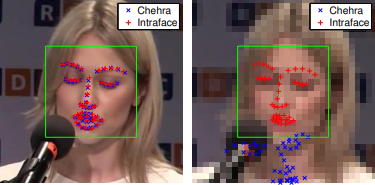
\includegraphics[width=0.8\textwidth]{media/ict/image15}
	\caption*{}
\end{figure}


{\bfseries Рис.1} - {\bfseries Сравнение обнаружения ориентиров на лице с
использованием Chehra и Intraface}

\emph{Пример детектирования морганий:}

- на рисунке 2 показано, как пороговый метод (EAR Threshold) может
ошибочно

фиксировать моргание во время движения головы или изменения выражения
лица;

- классификатор SVM успешно отличает такие случайные движения от
реальных

морганий, анализируя изменения коэффициента EAR в более длинной
временной последовательности.

\emph{Детектирование морганий при разных условиях}

Модель была протестирована в различных условиях, включая изменения
освещения, ношение очков и повороты головы. На изображении ниже показаны
скриншоты из видеоролика с участником, который носит очки. Несмотря на
присутствие очков, модель точно детектировала моргания. Это ещё раз
подчеркивает устойчивость метода к визуальным помехам и различным
условиям съёмки.

\emph{Пример работы модели на участниках с очками:}

- красные линии на изображении показывают автоматически детектированные

ориентиры глаз, которые помогают вычислить коэффициент EAR;

- даже при наличии очков, детектор ориентиров эффективно справляется с

локализацией глаз.

\begin{figure}[H]
	\centering
	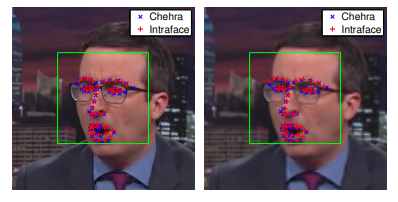
\includegraphics[width=0.8\textwidth]{media/ict/image16}
	\caption*{}
\end{figure}


{\bfseries Рис. 2 - Детектирования морганий}

Важным аспектом для работы модели в реальных условиях является её
устойчивость к поворотам головы и изменению угла зрения. На изображении
ниже показан пример работы модели, когда участник слегка поворачивает
голову в сторону. Как видно из графика EAR, даже при таких изменениях
положения головы, модель продолжает точно детектировать моменты
моргания.

\begin{itemize}
\item
  На изображении виден поворот головы участника относительно камеры.
\item
  Модель всё ещё успешно детектирует моргания благодаря инвариантности
  коэффициента EAR к изменениям масштаба и ориентации.
\end{itemize}

В ходе тестирования предложенной модели были получены следующие выводы:

- точность модели на различных наборах данных составила 90--99\%, в
зависимости от

условий съёмки и набора данных;

- классификатор SVM значительно улучшил точность по сравнению с простыми

пороговыми методами, особенно в сложных условиях, таких как улыбки,
ношение очков и изменения в положении головы;

-гибкость и устойчивость модели позволяют её использовать в широком
диапазоне приложений, начиная от мониторинга водителей для
предотвращения усталости, до использования в системах биометрической
идентификации и интерфейсах для людей с ограниченными возможностями.

\begin{figure}[H]
	\centering
	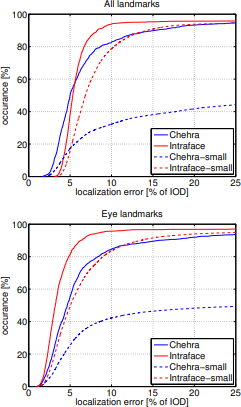
\includegraphics[width=0.8\textwidth]{media/ict/image17}
	\caption*{}
\end{figure}


{\bfseries Рис.3. - сравнивающих производительность систем обнаружения
ориентиров лица --- Chehra, Intraface, Chehra-small и Intraface-small}

На графиках представлены результаты сравнения точности определения
ключевых точек лица с помощью алгоритмов Chehra, Intraface, а также их
версий с уменьшенной моделью (Chehra-small и Intraface-small).

На первом графике показана ошибка локализации всех ключевых точек лица,
измеренная в процентах от межзрачкового расстояния (IOD). Чем выше
кривая, тем точнее модель. Видно, что Intraface и Chehra показывают
примерно схожую точность при малых ошибках, но Intraface имеет небольшое
преимущество. Уменьшенные версии моделей (Chehra-small и
Intraface-small) демонстрируют заметно худшие результаты, особенно при
значительных ошибках локализации.

На втором графике приведены данные только для ключевых точек глаз. Здесь
Intraface также имеет преимущество перед Chehra, особенно при низких
значениях ошибки локализации. Уменьшенные версии моделей также
показывают худшие результаты по сравнению с полными моделями, что
указывает на снижение точности при уменьшении размера модели.

Intraface демонстрирует лучшие результаты по сравнению с Chehra,
особенно на изображениях с низким разрешением. Это делает его более
подходящим для приложений, где важна высокая точность детекции
ориентиров даже при плохом качестве изображения.

{\bfseries Выводы.} Предложенная в статье модель для детектирования
морганий на основе коэффициента пропорции глаз (EAR) и классификатора
SVM демонстрирует высокую эффективность и применимость в задачах
реального времени. Модель основывается на детекторах лицевых ориентиров,
которые с высокой точностью распознают ключевые точки на лице, даже при
изменениях освещенности, выражений лица и поворотах головы. Это делает
модель устойчивой и адаптируемой к широкому спектру условий, что имеет
важное значение для различных приложений компьютерного зрения.

В этом исследовании представлен алгоритм для обнаружения морганий глаз в
режиме реального времени с использованием точек лицевых ориентиров. Он
находит применение в таких задачах, как мониторинг внимательности
оператора и предотвращение синдрома компьютерного зрения. Используя
современные детекторы ориентиров, исследование решает задачи, связанные
с изменениями положения головы, освещением и мимикой, что обеспечивает
надёжность и точность обнаружения морганий.

Основной вклад этой работы заключается в интеграции детекции лицевых
ориентиров с классификатором на основе машины опорных векторов (SVM) для
точного обнаружения морганий. Алгоритм использует новый признак --
коэффициент соотношения сторон глаза (EAR), который вычисляется на
основе положения ориентиров, чтобы оценить степень открытия глаза. Такой
подход превосходит передовые методы по производительности и скорости
работы в режиме реального времени на стандартных наборах данных.

Использованные в исследовании детекторы лицевых ориентиров достаточно
надёжны для отслеживания движений глаз в различных условиях. Их
способность точно улавливать изменения в открытии глаз обеспечивает
прочную основу для процесса детекции морганий. В работе подчёркивается
высокая точность и скорость этих детекторов, что имеет решающее значение
для приложений в реальном времени.

Предложенный алгоритм вычисляет коэффициент EAR на основе ориентиров и
обучает SVM для обнаружения морганий на последовательности кадров. Такая
комбинация повышает точность детекции морганий, учитывая временные
изменения, а не полагаясь только на отдельные изображения. Классификатор
SVM также различает моргания и другие движения глаз, такие как зевота
или намеренное закрытие глаз.

Одной из главных проблем предыдущих методов была их чувствительность к
условиям окружающей среды, таким как разрешение изображения или
ориентация головы. Это исследование демонстрирует, что использование
наборов данных, собранных в реальных условиях, позволяет методу детекции
ориентиров хорошо обобщать данные для различных сценариев, что повышает
надёжность системы обнаружения морганий.

В отличие от традиционных методов, основанных на оптическом потоке или
разнице интенсивности, предложенный метод использует более точный подход
на основе лицевых ориентиров. Это не только улучшает точность
обнаружения морганий, но и снижает вычислительную нагрузку, что делает
его подходящим для приложений в реальном времени.

Несмотря на высокую производительность алгоритма в большинстве условий,
допущение фиксированной продолжительности моргания является
ограничением. Так как у каждого человека моргание происходит по-разному,
адаптивный подход мог бы улучшить точность. Также использование
2D-оценки коэффициента открытия глаз может ограничить работу при
экстремальных поворотах головы, что требует рассмотрения 3D-подхода в
будущем.

В будущем исследовании можно сосредоточиться на улучшении адаптации
алгоритма к индивидуальным паттернам морганий и повышении точности
оценки состояния глаз при сильных поворотах головы. Также исследование
3D-методов детекции ориентиров может помочь решить проблемы, связанные с
вращениями головы, что ещё больше повысит надёжность системы.

{\bfseries Литература}

1. Кириллова Е.С., Сериков С.А. Интеллектуальная система безопасности
водителя, использующая обнаружение усталости // Международный журнал
гуманитарных и естественных наук.- 2024.- № 4-3 (91).- C.7-10. DOI
10.2441/2800-1000-2024-4-3-7-10

2. Кириллова Е.С., Сериков С.А. Методы и средства контроля состояния
водителя автомобиля // Международный журнал гуманитарных и естественных
наук. -2024. -№ 3-2 (90).- C.169-172. DOI
10.24412/2500-1000-2024-3-2-169-172

3. Булыгин А.О., Кашевник А.М.Анализ современных исследований в области
детектирования утомления водителя в кабине транспортного средства //
Системы анализа и обработки данных. - 2021. - № 3 (83).- С.19-36. DOI
10.17212/2782-2001-3-19-36

4. Лашков И.Б. Анализ поведения водителя при управлении транспортным
средством с использованием фронтальной камеры смартфона //
Информационно-управляющие системы.- 2017.- № 4. - C.7-18. DOI
10.15217/issn1684-8853.2017.4.7

5. Лашков, И.Б., Подход к распознаванию стиля вождения водителя
транспортного средства на основе использования сенсоров смартфона //
Информационно-управляющие системы.- 2018.- № 5.- С.2-12. DOI
10.31799/1684-8853-2018-5-2-12

6. Лобанова Ю. И. О возможностях прогноза аварийности водителей //
Психология. Психофизиология.- 2017.- № 10 (1).- C.74-87. DOI
10.14529/psy170108

7. Nasri I. et al. A Review of Driver Drowsiness Detection Systems:
Techniques, Advantages and Limitations. - 2022. DOI
10.48550/arXiv.2206.07489

8. Wu D. Improving automatic detection of driver fatigue and distraction
using machine learning.-2024.//arXiv preprint arXiv:2401.10213.

9. Singh Sengar S., Kumar A., Singh O. VigilEye-\/-Artificial
Intelligence-based Real-time Driver Drowsiness Detection.-2024. DOI
10.48550/arXiv.2406.15646

Jose J. et al. SleepyWheels: An Ensemble Model for Drowsiness Detection
leading to Accident Prevention.-2022. DOI 10.48550/arXiv.2211.00718

10.L. M. Bergasa, J. Nuevo, M. A. Sotelo, and M. Vazquez. Real-time
system for monitoring driver vigilance. In IEEE Intelligent Vehicles
Symposium, 2004
DOI~\href{https://doi.org/10.1109/IVS.2004.1336359}{10.1109/IVS.2004.1336359}.

11.T. Danisman, I. Bilasco, C. Djeraba, and N. Ihaddadene. Drowsy driver
detection system using eye blink patterns. In Machine and Web
Intelligence (ICMWI).2010.

DOI
\href{http://dx.doi.org/10.1109/ICMWI.2010.5648121}{10.1109/ICMWI.2010.5648121}

12.A. Sahayadhas, K. Sundaraj, and M. Murugappan. Detecting driver
drowsiness based on sensors: A review.// Sensors.-2012-Vol.12(12).-
P.16937-16953.\href{https://doi.org/10.3390/s121216937}{DOI
/10.3390/s121216937}

13.W. H. Lee, E. C. Lee, and K. E. Park. Blink detection robust to
various facial poses//Journal of Neuroscience Methods. - 2010.-
Vol.193(2):356-72.
DOI~\href{https://doi.org/10.1016/j.jneumeth.2010.08.034}{10.1016/j.jneumeth.2010.08.034}

14.Medicton group. The system I4Control. http:// www.i4tracking.cz/.
Date of address- 14.12.2024

15.D. Torricelli, M. Goffredo, S. Conforto, and M. Schmid. An adaptive
blink detector to initialize and update a view-basedremote eye gaze
tracking system in a natural scenario// Pattern Recognition Letters.-
2009.-Vol. 30(12).-P.1144
-1150.\href{https://doi.org/10.1016/j.patrec.2009.05.014}{DOI
/10.1016/j.patrec.2009.05.014}

{\bfseries References}

1.Kirillova E.S., Serikov S.A. Intellektual' naja sistema
bezopasnosti voditelja, ispol' zujushhaja obnaruzhenie
ustalosti // Mezhdunarodnyj zhurnal gumanitarnyh i estestvennyh nauk.-
2024.- № 4-3 (91).- C.7-10. DOI 10.2441/2800-1000-2024-4-3-7-10. {[}in
Russian{]}

2.Kirillova E.S., Serikov S.A. Metody i sredstva kontrolja sostojanija
voditelja avtomobilja // Mezhdunarodnyj zhurnal gumanitarnyh i
estestvennyh nauk. -2024. -№ 3-2 (90).- C.169-172. DOI
10.24412/2500-1000-2024-3-2-169-172 .{[}in Russian{]}

3.Bulygin A.O., Kashevnik A.M.Analiz sovremennyh issledovanij v oblasti
detektirovanija utomlenija voditelja v kabine transportnogo sredstva //
Sistemy analiza i obrabotki dannyh. - 2021. - № 3 (83).- S.19-36. DOI
10.17212/2782-2001-3-19-36. {[}in Russian{]}

4. Lashkov I.B. Analiz povedenija voditelja pri upravlenii transportnym
sredstvom s ispol' zovaniem frontal' noj
kamery smartfona // Informacionno-upravljajushhie sistemy.- 2017.- № 4.
- C.7-18. DOI 10.15217/issn1684-8853.2017.4.7. {[}in Russian{]}

5. Lashkov, I.B., Podhod k raspoznavaniju stilja vozhdenija voditelja
transportnogo sredstva na osnove ispol' zovanija sensorov
smartfona // Informacionno-upravljajushhie sistemy.- 2018.- № 5.-
S.2-12. DOI 10.31799/1684-8853-2018-5-2-12. {[}in Russian{]}

6. Lobanova Ju. I. O vozmozhnostjah prognoza avarijnosti voditelej //
Psihologija. Psihofiziologija.- 2017.- № 10 (1).- C.74-87. DOI
10.14529/psy170108. {[}in Russian{]}

7. Nasri I. et al. A Review of Driver Drowsiness Detection Systems:
Techniques, Advantages and Limitations. - 2022. DOI
10.48550/arXiv.2206.07489

8. Wu D. Improving automatic detection of driver fatigue and distraction
using machine learning.-2024.//arXiv preprint arXiv:2401.10213.

9. Singh Sengar S., Kumar A., Singh O. VigilEye-\/-Artificial
Intelligence-based Real-time Driver Drowsiness Detection.-2024. DOI
10.48550/arXiv.2406.15646

Jose J. et al. SleepyWheels: An Ensemble Model for Drowsiness Detection
leading to Accident Prevention.-2022. DOI 10.48550/arXiv.2211.00718

10.L. M. Bergasa, J. Nuevo, M. A. Sotelo, and M. Vazquez. Real-time
system for monitoring driver vigilance. In IEEE Intelligent Vehicles
Symposium, 2004
DOI~\href{https://doi.org/10.1109/IVS.2004.1336359}{10.1109/IVS.2004.1336359}.

11.T. Danisman, I. Bilasco, C. Djeraba, and N. Ihaddadene. Drowsy driver
detection system using eye blink patterns. In Machine and Web
Intelligence (ICMWI).2010.

DOI
\href{http://dx.doi.org/10.1109/ICMWI.2010.5648121}{10.1109/ICMWI.2010.5648121}

12.A. Sahayadhas, K. Sundaraj, and M. Murugappan. Detecting driver
drowsiness based on sensors: A review.// Sensors.-2012-Vol.12(12).-
P.16937-16953.\href{https://doi.org/10.3390/s121216937}{DOI
/10.3390/s121216937}

13.W. H. Lee, E. C. Lee, and K. E. Park. Blink detection robust to
various facial poses//Journal of Neuroscience Methods. - 2010.-
Vol.193(2):356-72.
DOI~\href{https://doi.org/10.1016/j.jneumeth.2010.08.034}{10.1016/j.jneumeth.2010.08.034}

14.Medicton group. The system I4Control. http:// www.i4tracking.cz/.
Date of address- 14.12.2024

15.D. Torricelli, M. Goffredo, S. Conforto, and M. Schmid. An adaptive
blink detector to initialize and update a view-basedremote eye gaze
tracking system in a natural scenario// Pattern Recognition Letters.-
2009.-Vol. 30(12).-P.1144
-1150.\href{https://doi.org/10.1016/j.patrec.2009.05.014}{DOI
/10.1016/j.patrec.2009.05.014}

\emph{{\bfseries Сведения об авторах}}

Танирбергенов А.Ж{\bfseries .}- и.о.доцент, заведующий кафедрой
криптологии, Евразийского национального университета им.Л. Н. Гумилева,
Астана, Казахстан, е-mail:
\href{mailto:t.adilbek@mail.ru}{\nolinkurl{t.adilbek@mail.ru}};

Серикбаева С.К. - PhD, старший преподаватель кафедры информационных
систем Евразийского национального университета им. Л. Н. Гумилева,
Астана, Казахстан, е-mail:
\href{mailto:inf_8585@mail.ru}{\nolinkurl{inf\_8585@mail.ru}};

Тасуов Б. - ассоцированный профессор кафедры Физика и информатика
Таразского регионального университета имени М.Х. Дулати, Тараз,
Казахстан, е-mail:
\href{mailto:b.tasuov@dulaty.kz}{\nolinkurl{b.tasuov@dulaty.kz}};

Мусагулова Г.Ш. - Кызылординский университет имени Коркыт Ата, старший
преподаватель образовательной программы «Информатика и
информационно-коммуникационные технологии», г. Кызылорда, Казахстан,
e-mail: \href{mailto:erkegulia@mail.ru}{\nolinkurl{erkegulia@mail.ru}};

Акзуллакызы Л. - Кызылординский университет имени Коркыт Ата, старший
преподаватель образовательной программы «Информатика и
информационно-коммуникационные технологии», г. Кызылорда, Казахстан,
e-mail: \href{mailto:la.z_1986@mail.ru}{\nolinkurl{la.z\_1986@mail.ru}};

Жарменова Б. К. - Кызылординский университет имени Коркыт Ата, старший
преподаватель образовательной программы «Информатика и
информационно-коммуникационные технологии», г. Кызылорда, Казахстан,
e-mail: \href{mailto:81_bota@mail.ru}{\nolinkurl{81\_bota@mail.ru}}

\emph{{\bfseries Information about authors}}

Tanirbergenov А.Adilbek - Acting Associate Professor, Head of the
Department of Cryptology, L.N. Gumilyov Eurasian National University,
Astana, Kazakhstan, е-mail:
\href{mailto:t.adilbek@mail.ru}{\nolinkurl{t.adilbek@mail.ru}};

Serikbayeva S. - PhD, Senior Lecturer of the Department of Information
Systems, L.N. Gumilyov Eurasian National University, Astana, Kazakhstan,
е-mail: \href{mailto:inf_8585@mail.ru}{\nolinkurl{inf\_8585@mail.ru}};

Tassuov B.- Associate Professor, Department of Physics and Informatics,
Taraz Regional University named after M.Kh. Dulaty, Taraz, Kazakhstan,
е-mail:
\href{mailto:b.tasuov@dulaty.kz}{\nolinkurl{b.tasuov@dulaty.kz}};

Mussagulova G. -, Korkyt Ata Kyzylorda University, senior lecturer of
the educational program "Informatics and Information Communication
Technologies", Kyzylorda, Kazakhstan,

e-mail: \href{mailto:erkegulia@mail.ru}{\nolinkurl{erkegulia@mail.ru}};

Akzullakyzy L{\bfseries .} - Korkyt Ata Kyzylorda University, senior
lecturer of the educational program "Informatics and Information
Communication Technologies", Kyzylorda, Kazakhstan,

e-mail: \href{mailto:laz_1986@mail.ru}{\nolinkurl{laz\_1986@mail.ru}};

Zharmenova B. - Korkyt Ata Kyzylorda University, senior lecturer of the
educational program "Informatics and Information Communication
Technologies", Kyzylorda, Kazakhstan,

e-mail: \href{mailto:81_bota@mail.ru}{\nolinkurl{81\_bota@mail.ru}}